\documentclass{article}

\usepackage[provide=*, magyar]{babel}

\usepackage{graphicx}
\usepackage{tikz}
\usepackage{pgfplots}

\pgfplotsset{compat=1.18}
\usetikzlibrary{calc}
\usepackage{calc}

\usetikzlibrary {arrows.meta}
\usepgfplotslibrary{fillbetween}

\usepackage{pdfpages}

\usepackage{amsmath}
\usepackage{siunitx}
\usepackage{tabularx}
\usepackage{booktabs}
\usepackage[table]{xcolor}
\usepackage{multicol}
\usepackage{footnote}

\makesavenoteenv{tabular}

\DeclareSIUnit\bar{bar}

\newcommand{\siunit}[2]{
	\SI{#1}{[#2]}
}

\newcommand{\n}[1]{
	\siunit{#1}{\newton}
}
\newcommand{\nmm}[1]{
	\siunit{#1}{\newton\mm}
}
\newcommand{\kn}[1]{
	\siunit{#1}{\kilo\newton}
}
\newcommand{\knm}[1]{
	\siunit{#1}{\kilo\newton\meter}
}
\newcommand{\mpa}[1]{
	\siunit{#1}{\mega\pascal}
}

\newcommand{\equal}[2]{
	\sum{#1} := 0 = #2
}

\newcommand{\circled}[1]{
	\raisebox{.5pt}{\textcircled{\raisebox{-.9pt} {#1}}}
}

\title{Dinamika HF1}

\date{\today}
\author{Vári Gergő (MQHJ0H)}


\begin{document}
	\pgfmathsetmacro\wtwoz{1.638}
\pgfmathsetmacro\wthreez{-7.878}

\pgfmathsetmacro\etwoz{16.613}

\pgfmathsetmacro\vstwo{0.56349}
\pgfmathsetmacro\vstwox{0.55}
\pgfmathsetmacro\vstwoy{-0.13}

\pgfmathsetmacro\astwo{1.4304}
\pgfmathsetmacro\astwox{-0.3103857094}
\pgfmathsetmacro\astwoy{-1.396187383}
\pgfmathsetmacro\astwoz{0}

\pgfmathsetmacro\astwot{0.017776}
\pgfmathsetmacro\astwon{1.4303}

\pgfmathsetmacro\pstwo{0.222}

\pgfmathsetmacro\lthree{0.04}

\pgfmathsetmacro\acce{1.862}

\pgfmathsetmacro\epstwo{16.613}
\pgfmathsetmacro\epsthree{-22.562}

\pgfmathsetmacro\alphatwo{80.826}

	\pagenumbering{gobble}

	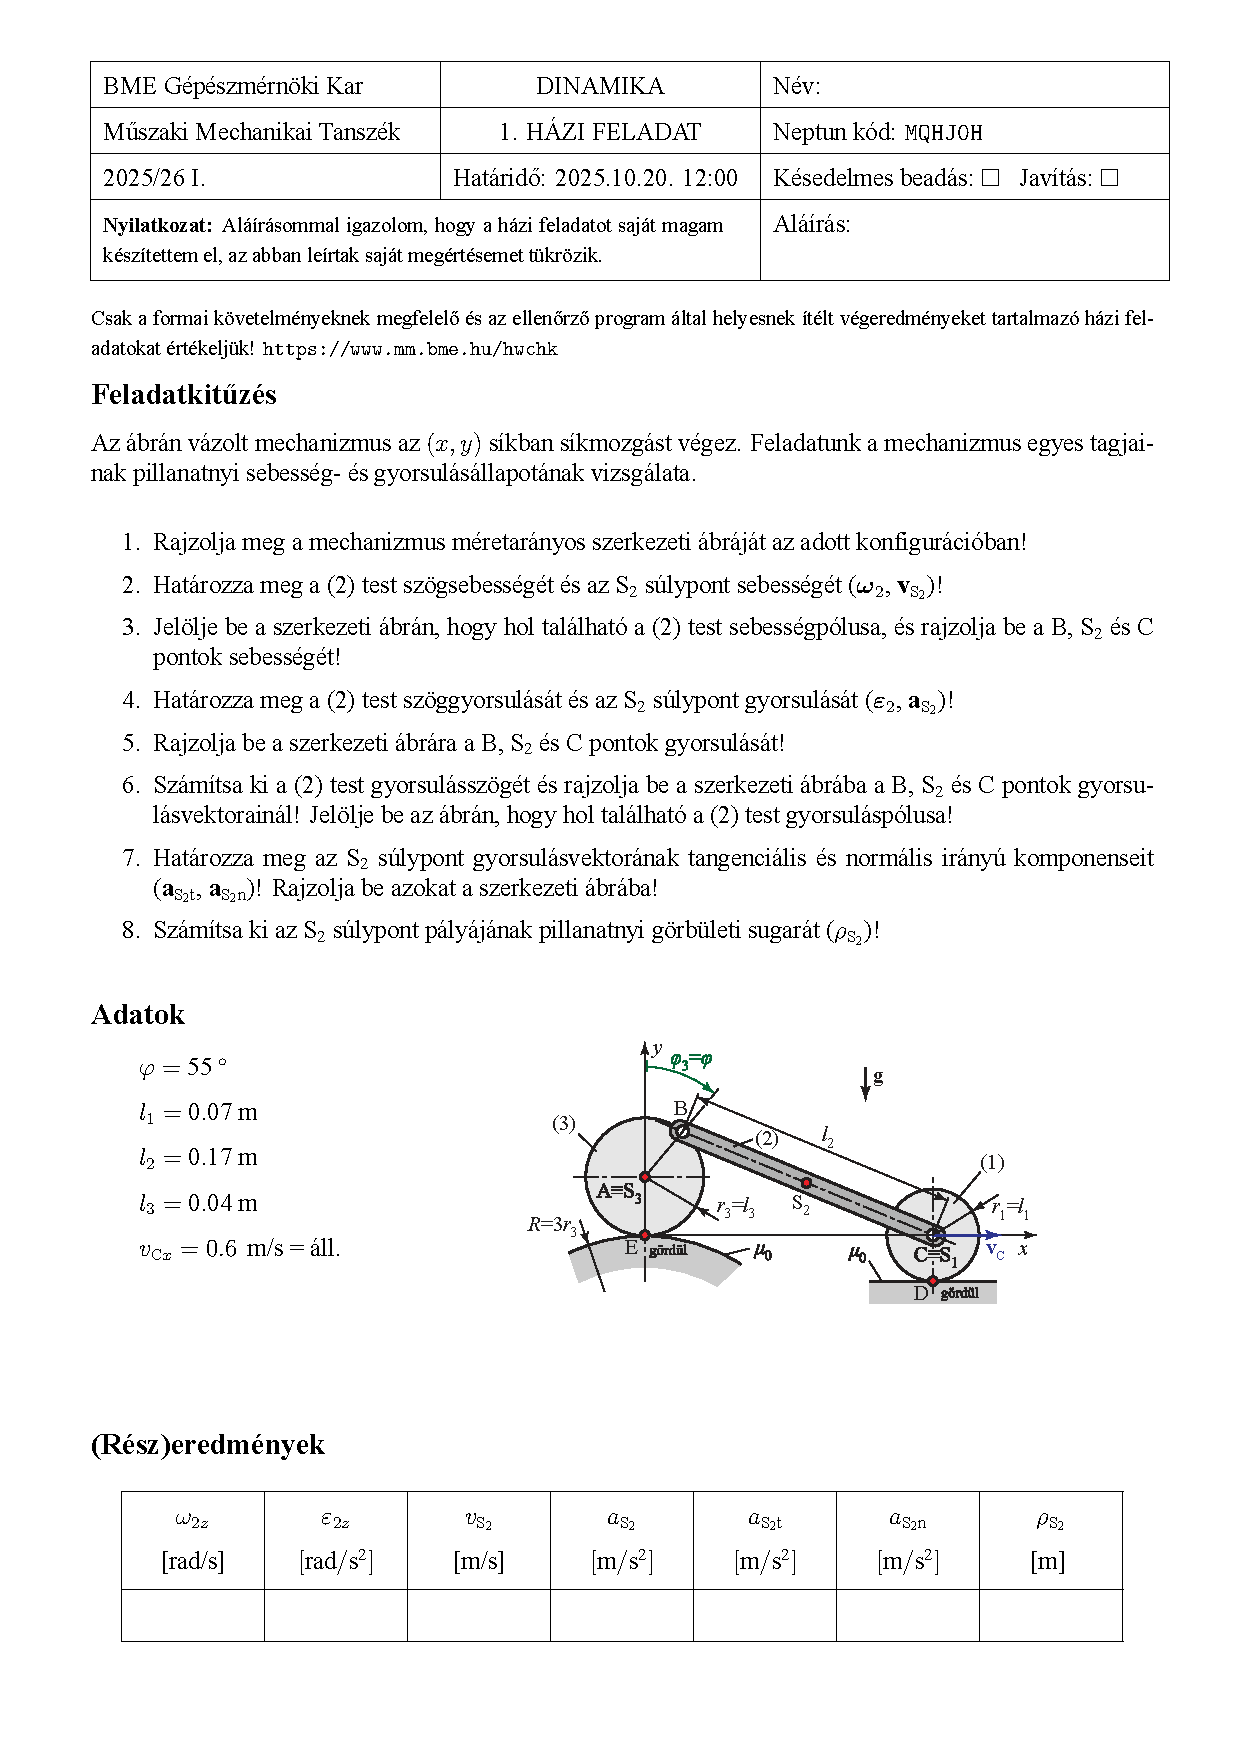
\includepdf[pages={1}, pagecommand={
	\begin{picture}(0,0) 
			\put(252, 93){Vári Gergő}
			\put(280, 21){\LARGE{Vári Gergő}}
			\put(-47, -600){\wtwoz}
			\put(14, -600){\etwoz}
			\put(75, -600){\vstwo}
			\put(144, -600){\astwo}
			\put(205, -600){\astwot}
			\put(274, -600){\astwon}
			\put(342, -600){\pstwo}
	\end{picture}
}]{exercise.pdf}


	\maketitle

	\rule{0pt}{100pt}
	\begin{figure}[hbt!]
		\centering
		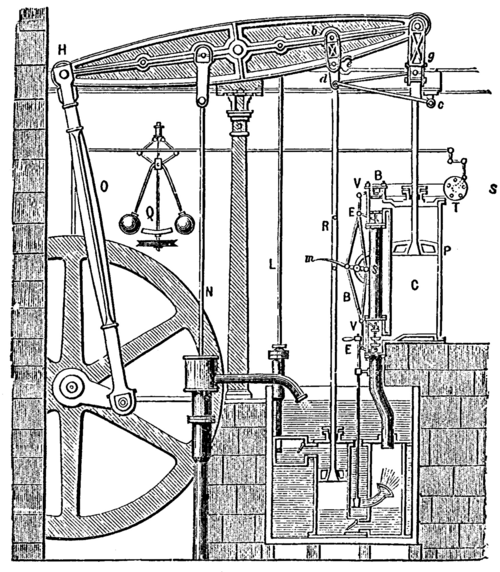
\includegraphics[scale=.45]{./images/assembly.png}
		\caption{Boulton \& Watt gőzgép}
	\end{figure}
	
	\newpage
	\tableofcontents

	\newpage
	\pagenumbering{arabic}

	\newpage
	\section{Szerkezeti ábra}

\structure


	\newpage
	\section{2-es test szög -és súlypontjának sebessége}

\subsection{Helyvektorok}
\begin{equation}
	\pmb{r}_\text{AB} =
	\begin{bmatrix}
		l_3 \sin\phi \\ l_3 \cos\phi \\ 0
	\end{bmatrix}
\end{equation}
\begin{equation}
	\pmb{r}_\text{CB} =
	\begin{bmatrix}
		-l_3 \cos\beta \\ l_3 \sin\beta \\ 0
	\end{bmatrix}
\end{equation}
\begin{align}
	&\sin\beta = \frac{l_3 + l_3\cos\phi}{l_2} \\
	&\pmb{r}_\text{CB} =
	\begin{bmatrix}
		-l_3 \cos\beta \\ l_3 \sin\beta \\ 0
	\end{bmatrix} \\
\end{align}
\begin{equation}
	\pmb{r}_{\text{C}{S_2}} = \frac{\pmb{r}_\text{CB}}{2}
\end{equation}
\begin{equation}
	\pmb{r}_\text{EA} = 
	\begin{bmatrix}
		0 \\ l_3 \\ 0
	\end{bmatrix}
\end{equation}

\subsection{Szögsebesség}
\begin{align}
	&\pmb{v}_\text{C} = 
	\begin{bmatrix}
		{v_\text{C}}_x \\ 0 \\ 0
	\end{bmatrix} \\
	&\pmb{v}_\text{E} = \pmb{0} \\
	&\pmb{v}_\text{A} = \pmb{v}_\text{E} + \pmb{\omega}_2 \times \pmb{r}_\text{EA} \\
	&\pmb{v}_\text{B} = 
	\pmb{v}_\text{C} + \pmb{\omega}_2 \times \pmb{r}_\text{CB} = 
	\pmb{v}_\text{A} + \pmb{\omega}_3 \times \pmb{r}_\text{AB} \Rightarrow \\
\end{align}
\begin{align}
	&\pmb{\omega}_2 = 
	\begin{bmatrix}
		0 \\ 0 \\ \wtwoz
	\end{bmatrix} \siunit{}{\radian\per\second} \\
	&\pmb{\omega}_3 = 
	\begin{bmatrix}
		0 \\ 0 \\ \wthreez
	\end{bmatrix} \siunit{}{\radian\per\second}
\end{align}

\subsection{Súlypont sebesség}
\begin{equation}
	\pmb{v}_{S_2} = \pmb{v}_\text{C} + \omega_2 \times \pmb{r}_{\text{C}{S_2}} = 
	\begin{bmatrix}
		\vstwox \\ \vstwoy \\ 0
	\end{bmatrix} \siunit{}{\m\per\second}
\end{equation}


	\newpage
	\section{Sebességpólus}

\subsection{Számítás}
A sebességpólusban $\pmb{0}$ a sebesség és ezzel megtalálhatjuk $\text{C}$-hez képesti helyvektorát.
\begin{align}
	&\pmb{v}_\text{C} = \pmb{v}_{P_2} + \pmb{\omega}_2 \times \pmb{r}_{{P_2}\text{C}} \Rightarrow \\
	&\pmb{r}_{{P_2}\text{C}} =
	\begin{bmatrix}
		0 \\ -0.365 \\ 0
	\end{bmatrix} \siunit{}{\m}
\end{align}

\subsection{Ábra}
\structurespeedpole


	\newpage
	\section{2-es test szög -és súlypontjának gyorsulása}

\subsection{Helyvektorok}
\begin{align}
	&\pmb{r}_\text{EA} = 
	\begin{bmatrix}
		0 \\ l_3 \\ 0
	\end{bmatrix} \\
	&\pmb{r}_\text{EB} = \pmb{r}_\text{EA} + \pmb{r}_\text{AB}
\end{align}

\subsection{Szöggyorsulás}
\begin{align}
	&\pmb{a}_\text{C} = \pmb{0} \\
	&v_\text{A} = r_3\omega_3 \\
	&{\pmb{a}_\text{A}}_y = - \frac{v_\text{A}^2}{R+r_3} \\
	&\pmb{a}_\text{A} = \pmb{a}_\text{E} + \pmb{\epsilon}_3 \times \pmb{r}_\text{EA} - \omega_3^2\pmb{r}_\text{EA} \Rightarrow \\
	&\pmb{a}_\text{E} =
	\begin{bmatrix}
		0 \\ \acce \\ 0
	\end{bmatrix} \siunit{}{\meter\per\second^2} \\
	&\pmb{a}_\text{B} 
	= \pmb{a}_\text{C} + \pmb{\epsilon_2} \times \pmb{r}_\text{CB} - \pmb{\omega}_2^2\pmb{r}_\text{CB}
\end{align}

\subsection{Súlypont gyorsulás}


	\newpage
	\section{Gyorsulásszög és gyorsuláspólus}

\subsection{Számítás}
\subsubsection{Gyorsulásszög}
\begin{equation}
	\alpha_2 = \text{arctg}{\frac{\epsilon_2}{\omega_2^2}} = \siunit{\alphatwo}{\degree}
\end{equation}

\subsubsection{Gyorsuláspólus}
\begin{equation}
	\pmb{a}_{G_2} = \pmb{0} = \pmb{a}_\text{C} \Rightarrow \text{G}_2 = C
\end{equation}

\subsection{Ábra}
\structureaccelerationpole


	\newpage
	\section{Gyorsulásvektor tangenciálisa és normálisa}

A sebességvektorból számolt tangenciális egységvektorral mindkét komponens megkapható.

\begin{align}
	&\pmb{e}_\text{t} = 
	\frac{\pmb{v}_{S_2}}{\left|\pmb{v}_{S_2}\right|} \\
	&\left| \pmb{a}_{{S_2}_t} \right| = 
	\pmb{a}_{S_2} \cdot \pmb{e}_\text{t} \\
	&\pmb{a}_{{S_2}_t} = 
	\left|\pmb{a}_{{S_2}_t}\right| \cdot \pmb{e}_\text{t} = 
	\begin{bmatrix}
		\astwotx \\ \astwoty \\ \astwotz
	\end{bmatrix} \siunit{}{\m\per\second^2} \\
	&\pmb{a}_{{S_2}_n} = \pmb{a}_{{S_2}} - \pmb{a}_{{S_2}_t} =
	\begin{bmatrix}
		\astwonx \\ \astwony \\ \astwonz
	\end{bmatrix} \siunit{}{\m\per\second^2}
\end{align}


	\newpage
	\section{Pillanatnyi görbületi sugár}

\begin{equation}
	\rho_{S_2} = \frac{\left|\pmb{v}_{S_2}\right|^2}{\left|\pmb{a}_{{S_2}_n}\right|} = \siunit{\rhostwo}{\m}
\end{equation}

\end{document}
